\section{Lista de equipos}

El primer problema que se plantea al intentar realizar un Análisis de
Equipos es elaborar una lista ordenada de los equipos que hay en ella.
Realizar un inventario de los activos de la planta es algo más complejo 
de lo que pueda parecer en un primer momento.

Una simple lista de todos los motores, bombas, sensores, etc., de la planta no es útil ni práctica.
Una lista de estas características no es más que una
lista de datos, no es información.


% Define block styles
\tikzstyle{block} = [rectangle, draw, fill=white!20, text centered, rounded corners]
\tikzstyle{line} = [draw, -latex']

\begin{figure}[h]
    \centering
    
\begin{tikzpicture}[ auto]
    % Place nodes
    \node [block] (plantas) {PLANTAS  (Nivel 1)};
    \node [block, below of=plantas] (areas) {AREAS (Nivel 2)};
    \node [block, below of=areas] (equipos) {EQUIPOS (Nivel 3)};
    \node [block, below of=equipos] (sistemas) {SISTEMAS (Nivel 4)};
    \node [block, below of=sistemas] (elementos) {ELEMENTOS (Nivel 5)};
    \node [block, below of=elementos] (componentes) {COMPONENTES (Nivel 6)};
    % Draw edges
    \path [line] (plantas) -> (areas);
    \path [line] (areas) -> (equipos);
    \path [line] (equipos) -> (sistemas);
    \path [line] (sistemas) -> (elementos);
    \path [line] (elementos) -> (componentes);
    
\end{tikzpicture}
    \caption{Niveles}
    \label{fig:my_label}
\end{figure}

Si queremos elaborar una lista de equipos
realmente útil, debemos expresar esta lista en forma de estructura arbórea, en
la que se indiquen las relaciones de dependencia de cada uno de los ítems con
los restantes.

En una planta industrial podemos distinguir los siguientes niveles, a la
hora de elaborar esta estructura arbórea:
Una empresa puede tener una o varias plantas de producción, cada una de
las cuales puede estar dividida en diferentes zonas o áreas funcionales. Estas
áreas pueden tener en común la similitud de sus equipos, una línea de producto 
determinada o una función. 

\begin{figure}
    \centering
    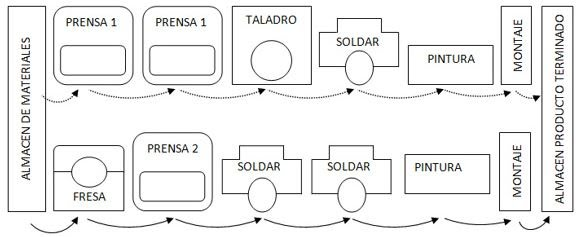
\includegraphics[width=0.5\textwidth]{images/03/layout2.JPG}
    \caption{Layout de planta.}
    \label{fig:my_layout2}
\end{figure}

Cada una de estas áreas estará formada por
un conjunto de equipos, iguales o diferentes, que tienen una entidad propia.
Cada equipo, a su vez, está dividido en una serie de sistemas funcionales, que
se ocupan de una misión dentro de él. Los sistemas, a su vez, se descomponen
en elementos (el motor de una bomba de lubricación será un elemento). Los
componentes son partes más pequeñas de los elementos, y son las partes
que habitualmente se sustituyen en una reparación.
Definamos en primer lugar qué entendemos por cada uno de estos términos:
\begin{enumerate}

\item Planta: Centro de trabajo. Ej.: Empresa Tenaris, Planta de Argentina, San Luis Villa Mercedes.

\item Área: Zona de la planta que tiene una característica común (centro de coste, similitud de equipos,
línea de producto, función). Ej.: Area Servicios Generales, Área hornos, Área Línea 1.

\item Equipo: Cada uno de las unidades productivas que componen el área, que
constituyen un conjunto único

\item Sistema: Conjunto de elementos que tienen una función común dentro de
un equipo.

\item Elemento: cada uno de las partes que integran un sistema. Ej.: el motor de
la bomba de lubricación de un compresor. Es importante diferenciar elemento y equipo. Un equipo puede estar conectado o dar servicio a más de un
equipo. Un elemento, en cambio, sólo puede pertenecer a un equipo. Si el
item que tratamos de identificar puede estar conectado o dar servicio simultáneamente a más de un equipo, será un equipo, y no un elemento. Así, si una
bomba de lubricación sólo lubrica un compresor, se tratará de un elemento del
compresor. Si, en cambio, se trata de una bomba que envía aceite de lubricación a varios compresores (sistema de lubricación centralizado), se tratará en
realidad de otro equipo, y no de un elemento de alguno de ellos.

\item Componentes: partes en que puede subdividirse un elemento. Ej.: Rodamiento de un motor, junta rascadora de un cilindro neumático.
    
\end{enumerate}


\actividad{Realizar, contestar e investigar}
\begin{enumerate}
    \item Copiar texto anterior en la parte de teoría de la carpeta.
    \item ¿Qué es un activo de una planta? ¿Qué es un inventario y para qué es necesario realizar un inventario de los activos?
    \item ¿Qué información debe contener una lista realmente útil?
    \item ¿Qué es una estructura arbórea? Dar ejemplos.
    \item Dar 2 ejemplos que contengan: Planta, Área, Equipo, Sistema, Elementos y componentes.
    
\end{enumerate}
